%=======================+=========================
%================  Introduction  ================
%=================================================
\section[The \gx{} experiment]{\label{sec:gluexexperiment} The \gx{} experiment}
The search for QCD exotics has been on going for several decades and utilizing data from a wide range of experiments and production mechanisms. Historically, such searches have looked for gluonic excitations of mesons, looking for both states of pure glue, glueballs, and those where the gluonic field binding the quark-anti-quark pair has been excited, hybrid mesons. Reviews of searches for glueballs~\cite{Crede:2008vw} show that most of these looked for so-called scalar glueballs, where the searches rely on over population of nonets as well as unusual decay patterns of the states. In the search for hybrid mesons~\cite{Meyer:2010ku,Meyer:2015eta}, searches have focused on states with non-quark-anti-quark (exotic) quantum numbers and good evidence exists for an isospin $1$ state, the $\pi_{1}(1600)$. Looking collectively at the past work, data from high-statistics photoproduction experiments in the relevant energy regime is lacking in these studies. 

\begin{figure}[h!]\centering
\includegraphics[width=0.75\textwidth]{figures/detector_beamline_noplug_dark.pdf}
\caption[]{\label{fig:gluex_cut-away}A cut-away drawing of the \GX{} detector in Hall D.}
\end{figure}
The GlueX experiment at Jefferson Lab has been built to both search for, and map out the spectrum of exotic hybrid mesons using a high-energy (9~GeV) linearly-polarized photon beam incident on a proton target\cite{gluex-ref}. The detector is nearly hermetic for both charged particles and photons, allowing for reconstruction of exclusive final states. A 2~T solenoidal magnet surrounds the drift-chamber based tracking. Two electromagnetic calorimeters cover the central and forward regions, and a down stream time-of-flight detector is provide particle identification capability through flight time measurements. The GlueX detector and beamline is shown schematically in Figure~\ref{fig:gluex_cut-away}.


\subsection[The Hall D complex]{The Hall D complex \label{sec:gluexexperiment:complex}}
The Hall D complex consists of a tagger hall where incident 12~GeV electrons produce
a beam of linearly polarized photons, and the experimental hall, where the photons interact
in an experimental target and the resulting interactions are recorded by the \GX{} detector.
A schematic of the complex, including the tagger area and the \GX{} experiment, is shown 
in Figure~\ref{fig:gluex_schematic}.

More information on the production, tagging and monitoring of the photon beam can be found in
Chapter~\ref{sec:chap:beam}. The \GX{} detector is described in detail in 
Chapter~\ref{sec:hall-d-spectrometer}.
\mysubsection[Experimental Description]{Experimental Description}
\label{sec:intro:detector}
As seen in Figure~\ref{fig:gluex_schematic}, the 12~GeV electron beam passes through a 
thin diamond wafer, where bremsstrahlung photons are produced. The electrons are then deflected
by the tagger magnet. Non-radiating electrons are sent to a beam dump, while the electrons which
have radiated more than a half of their energy
are detected by a pair of hodoscope arrays. These arrays are aligned such that each detector element
maps onto a narrow momentum range in the deflected electrons, and hence, a narrow energy range
in the produced photons. Thus, the energy of each photon is ``tagged'' and known in  the experiment.
The photon beam then travels about $80\, m$ to the experimental hall, where prior to entering the
experiment, it is collimated, and monitored using both a polarimeter and a pair spectrometer.

The photons can then interact in the target in \GX{}. Much of the experimental apparatus is inside
a solenoidal magnet with central field of 2~T. The charged particles produced by the interacting
photons are tracked by the start counter immediately outside the target (not shown in the figure),
and then a pair of tracking systems. The central drift chamber is based on 28 layers of axial and stereo
straws. The forward drift chambers are 24 drift chambers planes with both cathode
and anode readout.  The flight-time of charged
particles are measured using a combination of the start counter and the time-of-flight wall in the forward
direction, and the start counter and the barrel calorimeter inside the solenoid.

The final-state photons are detected in a pair of calorimeters. The barrel calorimeter, located inside the 
solenoid, consists if layers of scintillating fiber alternating with lead sheets. The forward calorimeter
is downstream of the time-of-flight wall, and consists of $2800$ lead-glass blocks. 

\subsection[Experimental Requirements]{Experimental Requirements \label{sec:intro:requirements}}
In order to be able to exclusively reconstruct events with final states given in Table~\ref{tab:exotic_modes},
accurate reconstruction of the incident photon, as well as the produced charge particles and photons
is necessary. 

The linear polarization of the incident photon beam is produced through the coherent 
bremsstrahlung process. These coherent photons have energies in the range of 8.4 to 9~GeV,
and will be about $40\%$, after the beam collimation to $\sim{}25~\mu$rad with respect to the incoming 
electron direction. For these linearly-polarized photons, it is necessary to accurately know the photon 
energy, both for the exclusive final state reconstruction and also to accurately determine the photon 
polarization on an event-by-event basis. In \GX{}, this energy is known to an accuracy of $0.1\%$ of the
incident photon energy.

In order to exclusively reconstruct multi-particle final states, the \GX{} detector needs be nearly
hermetic with good momentum and energy resolution for both charged particles and photons.
In order to be able to carry out the needed amplitude analysis, the detector acceptance  needs to 
be reasonably uniform, and well understood and modeled in simulation. Typical momentum resolution
for charged particles $1$--$2\%$, while for very-forward high-momentum particles, it is somewhat
worse at around $8$-$9\%$. For high-momentum charged particles, the tracking system has 
nearly hermetic acceptance for polar angles from about $2^{\circ}$ to $150^{\circ}$ in the lab. 
Because of target material, protons with momentum below about 350~MeV/c are not detected,
and pions with momentum under 200~MeV/c can have spiraling trajectories in the detector,
which make reconstruction challenging.

For photons, the typical energy resolution is $(5\,\mathrm{to}\,6\%)/\sqrt{E_{\gamma}}$. There is some 
variation in the barrel calorimeter resolution, depending on the incident angle of the photon,
but generally, photons above about 50~MeV are detected in the BCAL. The interaction point
along the beam direction is determined by comparing the information from the readouts on the 
upstream and downstream ends of the detector. The forward calorimeter can reconstruct photons
whose energy is larger than 100~MeV, with uniform resolution across the face of the detector.
There is an overlap region between the calorimeters at around $11^{\circ}$. Both photon detection 
efficiency and energy resolution is degraded in this region. 
 
\subsection{Data Requirements \label{sec:intro:data_requirements}}
In addition to the ability to reconstruct exclusive final states, the \GX{} experiment
will need to collect sufficient statistics to carry out amplitude analyses in small bins 
of meson invariant mass, and in momentum transfer, $|t|$. Large production cross
sections for reactions of interest are 10~$\mu$b, while more typical final-state 
cross sections are a few hundred nb. The \GX{} experiment has been built with a 
data acquisition system capable of collecting data using photon beams with $10^{8}~\gamma/$s
in the coherent peak. However, the experiment may be limited by electromagnetic backgrounds
in the detector, and force to run at photon  rates smaller than the design limit.

Expected raw event sizes are $15$kilobytes, and the data acquisition limit is expected to 
be 20~kHz. The level-1 hardware trigger alone will allow the experiment to run 
at in incident photon rate of $10^{7}~\gamma/$s in the coherent peak. Of the 20~kHz
event rate, about 2~kHz corresponds to hadronic interaction with photon in the coherent
peak. In order to run at higher beam intensities, the level-3 software trigger is needed to 
keep the rate of events to tape limited to 20~kHz. Including the events where the energy
of the interacting photon is above 9~GeV roughly doubles the number of interesting hadronic
events. 

The typical final states listed in Table~\ref{tab:exotic_modes} are expected to range from $3.5\%$ 
of the hadronic events for $\gamma p \rightarrow p 3\pi$ to under $1\%$. Assuming an $85\%$
reconstruction efficiency per final state particle, and that $60\%$ of the final state protons
are detectable, Table~\ref{tab:decay_rate_fractions} shows the number of reconstructed events per
hour assuming a total hadronic rate of 2~kHz for events with photon energies in the coherent
peak. These events are ultimately binned in both an meson invariant mass, as well as momentum
transfer, $|t|$, but for most of these channels $40$ days of running at $50\%$ efficiency would 
produce about a factor of $500$ times the number listed in the table.This is sufficient for
an initial amplitude analysis on many of these channels. Phase IV running of \GX{} anticipates 
$200$ days of running with $5\times  10^{7}$ photon beam intensity, a factor of $25$ over the
above estimate.

\begin{table}[h!]\centering
\caption[]{\label{tab:decay_rate_fractions}PYTHIA predictions for the fraction of hadronic events
in some final states interesting for exotic hybrid meson searches. The superscript on $(n\pi)^{0\pm}$
indicates the net electric charge of the $n$ pions. The specific final state column looks are one
particular charge combination, and the event rate column show the number of reconstructed events
per second assuming $10^{7}$ incident photons per second, and $85\%$ reconstruction efficiency
for each detected particle.}
\begin{tabular}{|l|r|l|r|}  \hline
Reaction & Fraction & Specific f.s. & Events/hour \\ \hline
$\gamma p \rightarrow p (3\pi)^{0}$ & $3.5\, \%$ & $p\pi^{+}\pi^{-}\pi^{0}$  & $87\times 10^{3}$ \\
$\gamma p \rightarrow n (3\pi)^{+}$ & $2.0\, \%$ & $n\pi^{+}\pi^{+}\pi^{-}$ & $58\times 10^{3}$ \\
$\gamma p \rightarrow p (2\pi)^{0}\omega$ & $1.8\, \%$ & $p2\pi^{+}2\pi^{-}\pi^{0}$ & $35\times 10^{3}$ \\
$\gamma p \rightarrow n (2\pi)^{+}\omega$ &  $1.0\, \%$ & $n2\pi^{+}\pi^{-}2\pi^{0}$ & $28\times 10^{3}$ \\
$\gamma p \rightarrow p (3\pi)^{0}\eta$ & $2.0\, \%$ & $p\pi^{+}\pi^{-}\pi^{0}\eta$ &  $14\times 10^{3}$ \\
$\gamma p \rightarrow n (3\pi)^{+}\eta$ &  $1.0\, \%$ & $n\pi^{+}\pi^{+}\pi^{-}\eta$ &  $7\times 10^{3}$ \\
$\gamma p \rightarrow p (2\pi)^{0}\eta$ & $1.0\, \%$ & $p\pi^{+}\pi^{-}\eta$ &  $8\times 10^{3}$ \\
$\gamma p \rightarrow n (2\pi)^{+}\eta$ &  $<1\, \%$ & $n\pi^{+}\pi^{0}\eta$ &  $<13\times 10^{3}$ \\
$\gamma p \rightarrow p \pi^{0}\omega$ & $<1\, \%$ & $p\pi^{+}\pi^{-}2\pi^{0}$ &  $<19\times 10^{3}$ \\
$\gamma p \rightarrow n \pi^{+}\omega$ &  $<1\, \%$ & $n2\pi^{+}\pi^{-}\pi^{0}$ &  $<33\times 10^{3}$ \\
\hline
\end{tabular} 
\end{table}


\subsection[Detector]{Detector \label{sec:detector}}
The design of the GlueX detector \cite{Ghoul:2015ifw} is based on a solenoidal magnet that surrounds all detectors in the central region, providing a magnetic field of about $2$~T along the direction of the photon beam, which impinges on a 
$30$~cm-long liquid hydrogen target.  A schematic of the detector including its major sub-detectors is given in Fig.\,\ref{fig:gluexsketch}.
\begin{figure}[tbp]
\begin{center}
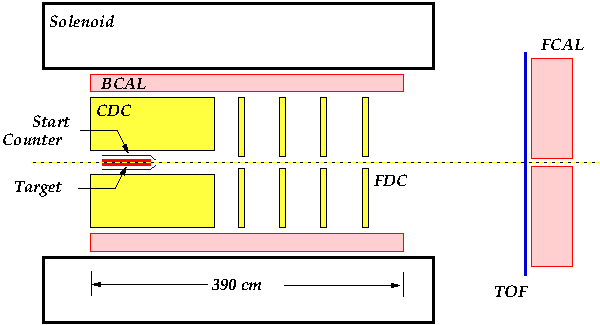
\includegraphics[width=0.7\textwidth]{figures/GlueX_Sketch.pdf}  
\caption{\label{fig:gluexsketch}          
  Sketch of GlueX detector.  The main systems of the detector are the Start Counter \cite{Pooser:2019rhu}, the Central Drift Chamber (CDC) \cite{VanHaarlem:2010yq} the Forward Drift Chamber (FDC) \cite{Pentchev2017281}, a scintillator-based Time of Flight (TOF) wall and a lead-glass Forward Calorimeter (FCAL) \cite{MORIYA201360}. The Barrel Calorimeter (BCAL) is sandwiched between the drift chambers and the inner radius of the solenoid.  (Color online)
}   
\end{center}  
\end{figure}

